% - starred version (e.g. \section*{Section name}) disables the (sub)section page.

\documentclass[czech]{beamer}
\usepackage{babel}

\usepackage{fontawesome5}

% use the focus theme (without fira)
\usetheme[nofirafonts]{focus}
\usefonttheme{serif}

% shamelessly stolen from https://www.patrickbaylis.com/posts/2018-10-11-beamer-resizing/
\usepackage{adjustbox}
\makeatletter
\newcommand{\fitimage}[2][\@nil]{
	\begin{figure}
		\begin{adjustbox}{width=0.9\textwidth, totalheight=\textheight-2\baselineskip-2\baselineskip,keepaspectratio}
			\includegraphics{#2}
		\end{adjustbox}
		\def\tmp{#1}%
	 \ifx\tmp\@nnil
			\else
			\caption{#1}
		\fi
	\end{figure}
}
\makeatother

\setlength{\belowcaptionskip}{-7pt}

% bullets
\setbeamertemplate{itemize item}{$\bullet$}
\setbeamertemplate{itemize subitem}{$\bullet$}
\setbeamertemplate{itemize subsubitem}{$\bullet$}
\setbeamercolor{itemize subsubitem}{fg=main}

% code
\usepackage{minted}
\setminted[python]{
	linenos,
	mathescape=true,
	escapeinside=||,
	autogobble,
	obeytabs=true,
	tabsize=4}

% strikethrough
\usepackage{soul}

% tables
\usepackage{booktabs}

% number lemmas and theorems
\setbeamertemplate{theorems}[numbered]

\makeatletter
\AtBeginEnvironment{proof}{\let\@addpunct\@gobble}
\makeatother

% translations
\newtranslation[to=Czech]{Definition}{Definice}

\usepackage{caption}
\usepackage{subcaption}

\title{Donjun}
\subtitle{generátor ASCII dungeonů}
\date{Tomáš Sláma \hfill \today}

\begin{document}
	\begin{frame}
		\maketitle
	\end{frame}
	
	\begin{frame}{Používání}
		\begin{figure}
		\centering
		\begin{minipage}{.5\textwidth}
			\centering
			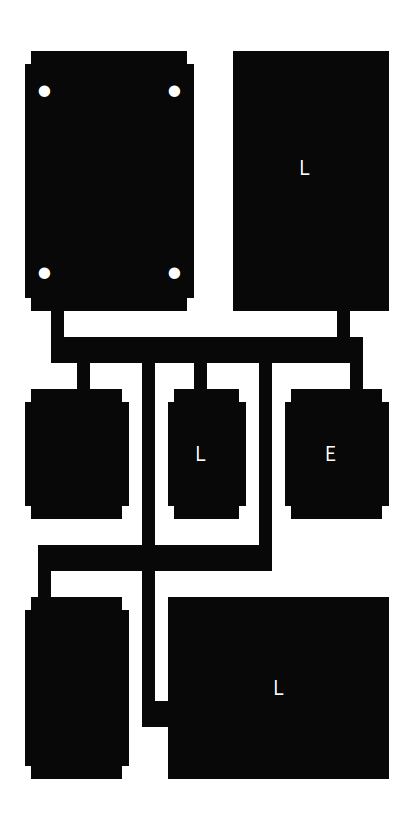
\includegraphics[width=.6\linewidth]{../img/30x30.png}
			\mintinline{text}{./Donjun -w 30 -h 30}
		\end{minipage}%
		\begin{minipage}{.5\textwidth}
			\centering
			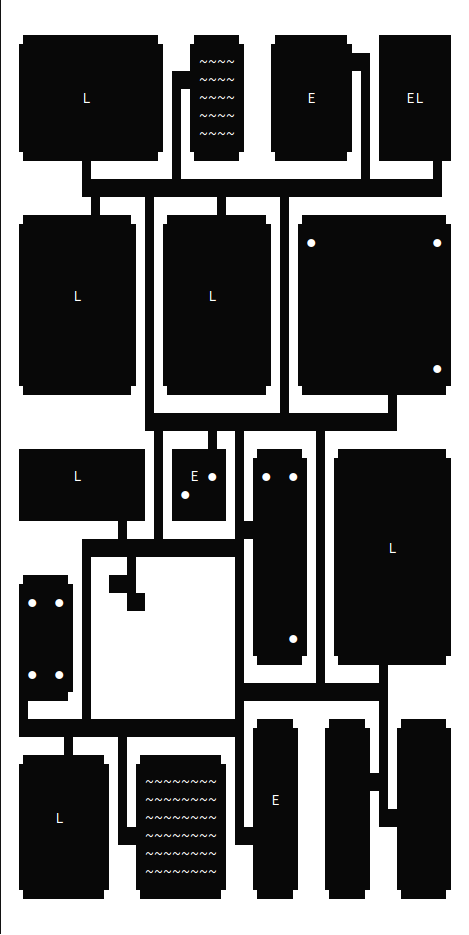
\includegraphics[width=.6\linewidth]{../img/50x50.png}
			\mintinline{text}{./Donjun -w 50 -h 50}
		\end{minipage}
		\end{figure}
	\end{frame}
	
	\begin{frame}{High-level overview}
		Důležitější třídy:
		\begin{itemize}
			\item \mintinline{text}{Constant.cs} -- konstanty algoritmů programu
			\item \mintinline{text}{Options.cs} -- option parsing; využívá \href{https://github.com/commandlineparser/commandline}{CommandLine}
			\item \mintinline{text}{Dungeon.cs} -- objekt produkovaný algoritmem
			\item \mintinline{text}{Generator.cs} -- generování částí dungeonu
			\item \mintinline{text}{Interface.cs} -- užitečné interfacy
			\item \mintinline{text}{Path.cs} -- objekt diskrétní cesty
			\item \mintinline{text}{Room.cs} -- objekt jedné místnosti dungeonu
		\end{itemize}
	\end{frame}
	
	\begin{frame}{Algoritmus}
		\begin{enumerate}
			\item rekurzivní generování místností dělením
			\begin{itemize}
				\item šance na horizontální/vertikální dělení
				\item proměnný poměr dělení
				\item dělení, dokud není místnost příliš malá (rozměry/objem)
			\end{itemize}
			\item spojování místností cestami
			\begin{itemize}
				\item přidej body stejně vzdálené od více místností
				\item odstraň mrtvé konce
			\end{itemize}
			\item generování samotných místností
			\begin{itemize}
				\item řada předem definovaných layoutů (častečně randomizovaných)
				\item šance na označení dané místnosti jako obsahující nepřátele/loot
			\end{itemize}
		\end{enumerate}
	\end{frame}

	\begin{frame}{Problémy}
		\begin{itemize}
			\item u ořezávání mrtvých konců se člověk nachytá
			\item správná parametrizace
			\item správné konstanty
			\item vhodný algoritmus pro generování místností
			\item závislost cest do místností a jejich layoutů
		\end{itemize}
	\end{frame}

\end{document}
